\task{6.1}{Verifying the upwind amplification calculation}
The amplification factor in the notes is
\[
G=1-\nu+\nu e^{-\ii\theta},\qquad \nu=\frac{c\Delta t}{\Delta x}.
\]
For real $\nu,\theta$, its complex conjugate is
$\overline G=1-\nu+\nu e^{\ii\theta}$. Therefore
\begin{align*}
|G|^2=G\overline G
&=(1-\nu)^2+\nu(1-\nu)(e^{\ii\theta}+e^{-\ii\theta})+\nu^2\\
&=(1-\nu)^2+2\nu(1-\nu)\cos\theta+\nu^2\\
&=1-2\nu+2\nu^2+2\nu(1-\nu)\cos\theta\\
&=1-2\nu(1-\nu)(1-\cos\theta).
\end{align*}
Use $1-\cos\theta=2\sin^2(\theta/2)$:
\[
\boxed{|G|^2=1-4\nu(1-\nu)\sin^2(\theta/2).}
\]
If $0\le\nu\le1$, the subtracted term is nonnegative, hence $|G|^2\le1$ for every wave number.
If $\nu<0$ or $\nu>1$, then $\nu(1-\nu)<0$, and choosing $\theta=\pi$ makes $|G|^2>1$.
Thus the condition is both necessary and sufficient for this Fourier analysis:
\[
\boxed{0\le\nu\le1.}
\]
At $\nu=1$ the method shifts the data by one cell per step, giving $|G|=1$ without numerical
damping. At $\nu=0$ the data do not move.

\task{6.2}{Von Neumann analysis in one dimension}
\partsol{a}
The one-dimensional heat scheme is
\[
u_j^{n+1}=u_j^n+r_x(u_{j+1}^n-2u_j^n+u_{j-1}^n).
\]
Substitute the Fourier mode $u_j^n=G^ne^{\ii j\theta}$.
A shift of one node multiplies the mode by $e^{\pm\ii\theta}$, so cancellation of the common
factor gives
\begin{align*}
G&=1+r_x(e^{\ii\theta}-2+e^{-\ii\theta})\\
&=1+2r_x(\cos\theta-1)\\
&=\boxed{1-4r_x\sin^2(\theta/2).}
\end{align*}
For the zero-amplification case this algebra is understood as substitution into the linear
one-step operator rather than division by a possibly zero factor at later time levels.
Since $r_x$ and $\sin^2(\theta/2)$ are real, $G$ is real.

\partsol{b}
For $r_x\ge0$, the amplification factor ranges between
\[
G(0)=1,\qquad G(\pi)=1-4r_x.
\]
The maximum absolute amplification is therefore
\[
\boxed{\max_\theta|G(\theta)|=\max\{1,|1-4r_x|\}.}
\]
This distinction matters: within the stable range, the constant mode $\theta=0$ already has
$|G|=1$. The high-frequency mode $\theta=\pi$ is the mode that first violates stability as
$r_x$ increases. Its spatial pattern is
\[
e^{\ii j\pi}=(-1)^j:\qquad +1,-1,+1,-1,\ldots
\]
This is the shortest alternating wavelength representable on the grid.

\partsol{c}
The upper bound $G\le1$ is automatic for $r_x\ge0$. The lower bound $G\ge-1$ for every
wave number requires
\[
1-4r_x\ge-1
\quad\Longrightarrow\quad r_x\le\frac12.
\]
Thus
\[
\boxed{0\le r_x=\frac{\alpha\Delta t}{\Delta x^2}\le\frac12,
\qquad \Delta t\le\frac{\Delta x^2}{2\alpha}.}
\]
At equality the alternating mode has $G=-1$, so its magnitude is bounded but it flips sign
at every time step. A slightly smaller step damps this mode. The bound is the standard
grid-independent Fourier limit; Task 6.5 explains a small finite-Dirichlet-grid distinction.

\task{6.3}{Von Neumann analysis in two dimensions}
\partsol{a}
Use $u_{j,k}^n=G^n e^{\ii(j\theta+k\phi)}$, where $j$ indexes $x$ and $k$ indexes $y$.
Inserting this into the general-spacing scheme gives
\begin{align*}
G(\theta,\phi)
&=1+r_x(e^{\ii\theta}-2+e^{-\ii\theta})
+r_y(e^{\ii\phi}-2+e^{-\ii\phi})\\
&=\boxed{1-4r_x\sin^2(\theta/2)-4r_y\sin^2(\phi/2).}
\end{align*}
The two directional contributions add because the discrete Laplacian is a sum of independent
$x$ and $y$ second differences.

\partsol{b}
For nonnegative $r_x,r_y$, $G\le1$. Its minimum is reached when both sine-squared factors
equal one, at $\theta=\phi=\pi$:
\[
G_{\min}=1-4(r_x+r_y).
\]
This spatial mode is $(-1)^{j+k}$: adjacent horizontal and vertical nodes have opposite signs,
forming a checkerboard. The maximum absolute factor is
$\max\{1,|1-4(r_x+r_y)|\}$, so this checkerboard is the stability-limiting mode.

Require its factor to be at least $-1$:
\[
1-4(r_x+r_y)\ge-1
\quad\Longleftrightarrow\quad r_x+r_y\le\frac12.
\]
Substitute the definitions of $r_x,r_y$:
\[
\boxed{\alpha\Delta t\left(\frac1{\Delta x^2}+\frac1{\Delta y^2}\right)\le\frac12,}
\]
or equivalently
\[
\boxed{\Delta t\le
\frac{1}{2\alpha(\Delta x^{-2}+\Delta y^{-2})}
=\frac{\Delta x^2\Delta y^2}{2\alpha(\Delta x^2+\Delta y^2)}.}
\]
The smaller mesh spacing is especially restrictive because it appears through its inverse square.

\partsol{c}
If $\Delta x=\Delta y=h$, then $r_x=r_y=r$ and
\[
G=1-4r\bigl(\sin^2(\theta/2)+\sin^2(\phi/2)\bigr).
\]
The condition becomes $2r\le1/2$, hence
\[
\boxed{0\le r=\frac{\alpha\Delta t}{h^2}\le\frac14,
\qquad \Delta t\le\frac{h^2}{4\alpha}.}
\]
At $r=1/4$ the ideal checkerboard has $G=-1$; choosing $r<1/4$ gives a safety margin.
This is the bound enforced in the ordinary solver runs.

\partsol{d}
For the same $h$ and $\alpha$, the 1D limit is $h^2/(2\alpha)$ and the 2D limit is
$h^2/(4\alpha)$: the admissible step is halved in 2D.
For three equal spacings, the additional directional term gives
\[
G=1-4r\left[\sin^2(\theta/2)+\sin^2(\phi/2)+\sin^2(\psi/2)\right].
\]
The minimum is $1-12r$, so stability requires
\[
\boxed{r\le\frac16\quad\text{in 3D}.}
\]
In $d$ dimensions with equal spacing, the same argument gives $r\le1/(2d)$.

\task{6.4}{Positivity of the weights and the maximum principle}
The equal-spacing weights from Task 5.3 are
\[
w_0=1-4r,\qquad w_1=w_2=w_3=w_4=r.
\]
They sum to one for every $r$, but they are all nonnegative only when
\[
r\ge0,\qquad 1-4r\ge0.
\]
Thus
\[
\boxed{0\le r\le\frac14.}
\]
This agrees with the Fourier stability bound in Task 6.3. For unequal spacings, the centre
weight is $1-2r_x-2r_y$ and the four neighbour weights are $r_x,r_x,r_y,r_y$.
Their nonnegativity yields $r_x+r_y\le1/2$, again the same condition.

\textbf{Why nonnegative weights imply boundedness.}
If the old stencil values lie between $m$ and $M$, then each nonnegative weighted value satisfies
$w_km\le w_ku_k\le w_kM$. Summing and using $\sum w_k=1$ gives
\[
m\le\sum_k w_ku_k\le M.
\]
Therefore no interior update creates a new maximum or minimum. By induction, with fixed
Dirichlet boundary temperatures the full solution remains between the initial and boundary
extrema. The same argument applied to the difference of two solutions establishes a maximum-norm
stability bound.

\textbf{What fails above the limit.}
If $r>1/4$, the coefficient of the old centre is negative, so the update is no longer a convex
average. For example, an old centre of $1$ surrounded by four zeros gives
\[
u_{\mathrm{centre}}^{n+1}=1-4r<0.
\]
A nonnegative temperature field can therefore become negative in a single step. Conversely,
a zero centre with four neighbours equal to one updates to $4r>1$.
These undershoots and overshoots are unphysical for this source-free diffusion problem.
The high-frequency error can then reverse sign and increase in magnitude, producing the
checkerboard instability. Some particular initial fields may remain harmless for a while;
the violated bound means there is no general stability guarantee.

\task{6.5}{Eigenvalues of the discrete second derivative (optional)}
We solve the optional exercise as an independent check of the 1D stability analysis.
Let $h=\Delta x=L/N$ and impose $u_0=u_N=0$.
For the semi-discrete heat equation $\bm u'=-A\bm u$, the matrix is
\[
A=\frac{\alpha}{h^2}
\begin{pmatrix}
2&-1&0&\cdots&0\\
-1&2&-1&\ddots&\vdots\\
0&-1&2&\ddots&0\\
\vdots&\ddots&\ddots&\ddots&-1\\
0&\cdots&0&-1&2
\end{pmatrix}.
\]
If one defines $A$ for $-D_2$ alone, omit $\alpha$ in its eigenvalues and multiply by $\alpha$
when applying them to the heat equation. Here $A$ includes diffusivity.

\partsol{a}
For $m=1,\ldots,N-1$, define
\[
v_i^{(m)}=\sin\!\left(\frac{m\pi i}{N}\right),\qquad
\theta_m=\frac{m\pi}{N}.
\]
Use $\sin(a+b)+\sin(a-b)=2\sin a\cos b$ to obtain
\begin{align*}
(Av^{(m)})_i
&=\frac{\alpha}{h^2}\left(2v_i^{(m)}-v_{i-1}^{(m)}-v_{i+1}^{(m)}\right)\\
&=\frac{\alpha}{h^2}(2-2\cos\theta_m)v_i^{(m)}\\
&=\frac{4\alpha}{h^2}\sin^2(\theta_m/2)v_i^{(m)}.
\end{align*}
The boundary components are zero, since $\sin0=\sin(m\pi)=0$, so the argument also holds
for the first and last interior equations. Therefore
\[
\boxed{\mu_m=\frac{4\alpha}{h^2}\sin^2\!\left(\frac{m\pi}{2N}\right).}
\]
All these eigenvalues are positive, as expected for $A$.

\partsol{b}
The sine-squared factor increases over $m=1,\ldots,N-1$, giving
\begin{align*}
\mu_{\max}=\mu_{N-1}
&=\frac{4\alpha}{h^2}\sin^2\!\left(\frac{(N-1)\pi}{2N}\right)\\
&=\boxed{\frac{4\alpha}{h^2}\cos^2\!\left(\frac{\pi}{2N}\right).}
\end{align*}
As $N\to\infty$, the cosine tends to one, so
$\mu_{\max}\sim4\alpha/h^2$. Thus the fastest discrete decay rate grows like $h^{-2}$.

\partsol{c}
Theorem 4.2 requires $\Delta t\le2/\mu_{\max}$, hence on this \emph{fixed finite Dirichlet grid}
\[
\boxed{\Delta t\le\frac{h^2}{2\alpha\cos^2(\pi/(2N))}.}
\]
This is slightly less restrictive than $h^2/(2\alpha)$ because
$\cos^2(\pi/(2N))<1$. There is no exact $\theta=\pi$ Fourier eigenvector among the
finite Dirichlet sine modes; the highest allowed frequency lies just below it.
As $N$ increases the difference disappears, recovering Task 6.2's standard bound.
The simpler bound $r_x\le1/2$ is valid for every $N$ and also guarantees nonnegative weights.

\partsol{d}
For fixed small $m$ and large $N$, use $\sin z=z-z^3/6+O(z^5)$:
\begin{align*}
\mu_m
&=\frac{4\alpha}{h^2}\left[
\left(\frac{m\pi h}{2L}\right)^2
-\frac13\left(\frac{m\pi h}{2L}\right)^4+O(h^6)\right]\\
&=\boxed{\alpha\left(\frac{m\pi}{L}\right)^2
-\frac{\alpha m^4\pi^4}{12L^4}h^2+O(h^4).}
\end{align*}
The exact 1D mode decays at rate $\alpha(m\pi/L)^2$, so the discrete rate converges to it
with second-order spatial error. The discrete rate is slightly smaller for well-resolved modes.
In 2D the rates add in the two directions, matching the separation-of-variables solution
from Task 1.3 in the refinement limit.

\task{6.6}{Counting the computational work}
Here the domain is the unit square, $\alpha=1$, $h=1/N$, and the largest standard stable step is
\[
\Delta t=\frac{h^2}{4}=\frac{1}{4N^2}.
\]

\partsol{a}
There are $N+1$ nodes along each direction, hence
\[
\boxed{\text{total nodes}=(N+1)^2,\qquad \text{updated interior nodes}=(N-1)^2.}
\]
To reach $T=0.1$ would require
\[
\frac{T}{\Delta t}=0.4N^2.
\]
If this is an integer, use exactly that many steps. Otherwise choose
\[
\boxed{M=\lceil0.4N^2\rceil,\qquad \Delta t_{\mathrm{used}}=0.1/M,}
\]
so the final time is exact and the stability limit is respected. The step count grows like $N^2$.

\partsol{b}
Using seven operations per updated node from Task 5.2(d),
\[
\boxed{W(N)=7(N-1)^2\lceil0.4N^2\rceil\sim2.8N^4\ \text{floating-point operations}.}
\]
Boundary assignment, initialization, output, index arithmetic, and loop control are not included
in this useful-operation count.

\partsol{c}
Doubling $N$ approximately quadruples the number of unknowns and quadruples the number of
time steps. Therefore, assuming the same sustained useful-operation rate,
\[
\boxed{\text{run-time factor}\simeq4\times4=16.}
\]
The exact ratio has small finite-$N$ and integer-rounding corrections. Hardware effects can
also change the sustained rate, so $16$ is the leading cost prediction.

\partsol{d}
At a sustained rate of $10^9$ useful operations per second,
\[
t_{\mathrm{estimate}}=\frac{W(N)}{10^9}.
\]
For the requested sizes:
\begin{center}
\begin{tabular}{rrrr}
\toprule
$N$ & Steps & Useful operations & Estimated time\\
\midrule
1000 & $400000$ & $2.7944028\times10^{12}$ & $2794.4\,\mathrm{s}\simeq46.6\,\mathrm{min}$\\
4000 & $6400000$ & $7.164416448\times10^{14}$ & $716441.6\,\mathrm{s}\simeq8.29\,\mathrm{days}$\\
\bottomrule
\end{tabular}
\end{center}
The asymptotic $2.8N^4$ formula gives $2800$ seconds and $716800$ seconds, respectively,
which are close to the exact-count estimates. Increasing $N$ by four multiplies the leading
work by $4^4=256$. These figures are estimates under the rate specified in the question,
not measured timings of the supplied program.

\task{6.7}{Breaking the stability condition on purpose}
\textbf{Experimental setup.}
We use the serial C++ implementation on a $65\times65$ node grid ($N=64$ intervals), with
$\alpha=1$. Initially the interior is zero and all four boundary edges are held at one.
No artificial perturbation is added. This boundary-heated test supplies spatial detail that
can excite unstable high-frequency modes.

The ordinary 2D bound and the deliberately excessive step are
\[
\Delta t_{\max}=\frac{1}{4\cdot64^2}=6.103515625\times10^{-5},
\]
\[
\boxed{\Delta t_{\mathrm{bad}}=1.05\Delta t_{\max}
=6.40869140625\times10^{-5},\qquad r=0.2625.}
\]
This unstable run uses a separate explicit experimental override. Ordinary solver runs reject
$r>1/4$. Each snapshot is computed from the same initial field for the indicated number of steps.

\textbf{Computed extrema.}
\begin{center}
\begin{tabular}{rrrr}
\toprule
Steps & Physical time & Minimum temperature & Maximum temperature\\
\midrule
\tableinput{tables/task_6_7.tex}
\bottomrule
\end{tabular}
\end{center}
The physically allowed range is $[0,1]$. At step 120 the maximum already exceeds one.
By step 160 large negative and positive temperatures have appeared, and by step 200 their
magnitudes are approximately $300$. The initial apparently plausible behaviour therefore does
not establish stability.

\begin{figure}[H]
\centering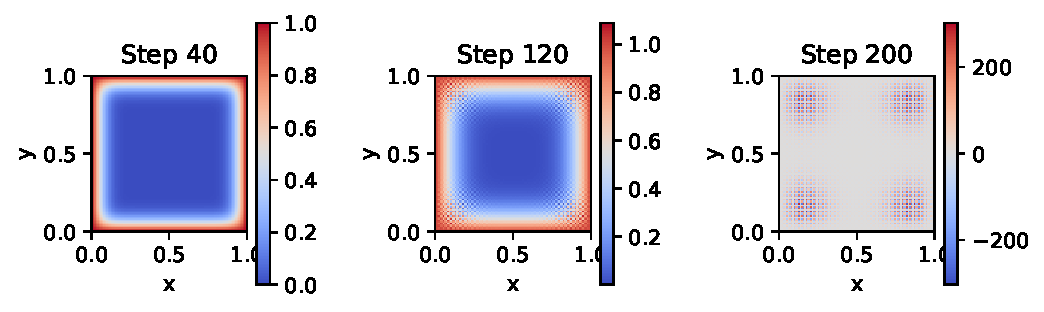
\includegraphics[width=\linewidth]{task_6_7_instability.pdf}
\caption{Instability at $r=0.2625$. Each panel has its own colour scale.
The early heat front looks reasonable; later panels show alternating grid-scale errors and growing extrema.}
\end{figure}
\textbf{Where it appears and what it looks like.}
In this experiment the visible oscillations first emerge in the boundary-heated regions near
the corners, before spreading farther into the plate. At step 120 a maximum occurs at grid
index $(i,j)=(4,59)$, near the upper-left corner. Symmetry produces equivalent regions near
the other corners, up to rounding. Alternating high and low values on neighbouring nodes form
a checkerboard. The location is specific to the initial and boundary data: if high-frequency
noise were inserted throughout the interior, the instability could appear there instead.

\begin{figure}[H]
\centering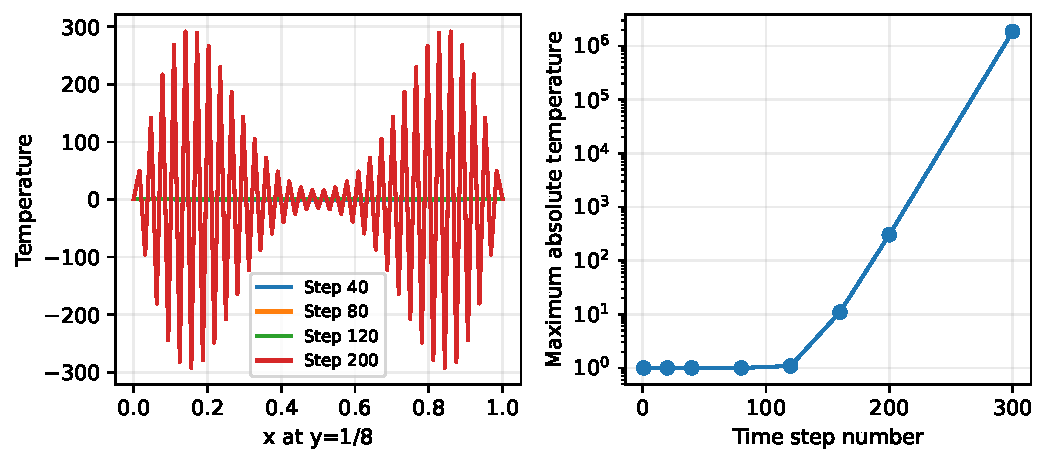
\includegraphics[width=\linewidth]{task_6_7_growth.pdf}
\caption{A horizontal cut at $y=1/8$ shows alternating values, while the maximum magnitude
eventually grows rapidly. Boundary values remain fixed at one throughout.}
\end{figure}
\textbf{Connection with the Fourier calculation.}
Task 6.3 gives the ideal checkerboard factor
\[
G(\pi,\pi)=1-8r=1-8(0.2625)=-1.1.
\]
Thus a checkerboard perturbation changes sign and grows by approximately $10\%$ each step.
After $n$ steps, its amplitude behaves like $(-1.1)^n$ in the Fourier model.
For the finite Dirichlet grid the highest sine mode instead has
\[
G_{\mathrm{highest}}=1-8r\cos^2\!\left(\frac{\pi}{2N}\right)
\simeq-1.09874\quad(N=64),
\]
which is still unstable. Its envelope and the superposition of nearby modes explain why the
actual field is not a uniform-amplitude checkerboard. Once this high-frequency component
dominates, the computation no longer represents heat diffusion.
